\documentclass[12pt,letterpaper]{article}


\newcommand{\studentname}{Ben Bassett}
\newcommand{\labpartner}{Katrina Sumarli}

\title{\textsc{Lab 04: Modes of a Beaded Cord}}
\newcommand{\shorttitle}{Modes of a Beaded Cord}

\newcommand{\course}{PHY310}
\newcommand{\labdate}{10-1-2024}

%------------------------------------------------------------------------------------------------------------

\usepackage[letterpaper,left=1in,right=1in,bottom=1in,top=1in]{geometry}
\usepackage{fancyhdr}
\usepackage{subfigure}
\usepackage{graphicx}
\usepackage{amsmath}
\usepackage{cleveref}
\usepackage{booktabs}
\usepackage[british]{babel}
\usepackage[square,comma,numbers,sort&compress]{natbib}
\usepackage{csvsimple}
\usepackage{graphicx}
\usepackage{pgfplotstable}
\usepackage{textcomp,gensymb}
\usepackage{array}
\usepackage{tabu}
\usepackage{multirow}
\usepackage{url}
\usepackage{lipsum}
\usepackage{dsfont}
\pgfplotsset{compat=1.9}% supress warning
\begin{document}

%------------------------------------------------------------------------------------------------------------

\setlength{\parindent}{1em}
\setlength{\parskip}{0.5em}
\author{\course~Lab Journal \\ \\ \studentname\,\& \labpartner}
\date{\labdate}

\renewcommand\abstractname{Summary}

\pagestyle{fancy}
\fancyhead{}
\fancyhead[l]{\course:~\shorttitle}
\fancyhead[r]{\studentname}
\fancyfoot{}
\fancyfoot[C]{\thepage}
\renewcommand{\headrulewidth}{0pt}
\renewcommand{\footrulewidth}{0pt}

\renewcommand\bibname{References}

%------------------------------------------------------------------------------------------------------------

\renewcommand\abstractname{Abstract}
\maketitle

% COMMENT IN IF ASKED TO SUBMIT REPORT WITH ABSTRACT
%\begin{abstract}
%Maximum 200 words.
%\end{abstract}

\section{Purpose}
This lab aimed to measure the dispersion of waves on a beaded string under tension.

\section{Experimental Apparatus}

We were given a length of string with 9 beads affixed every 10 cm, a mechanical wave driver, a large and small mounted retort stand, a pulley, ruler, and various weights (including hanger). Our general setup is illustrated in Figure \ref{fig:setup}.

\begin{figure}[h]
    \centering
    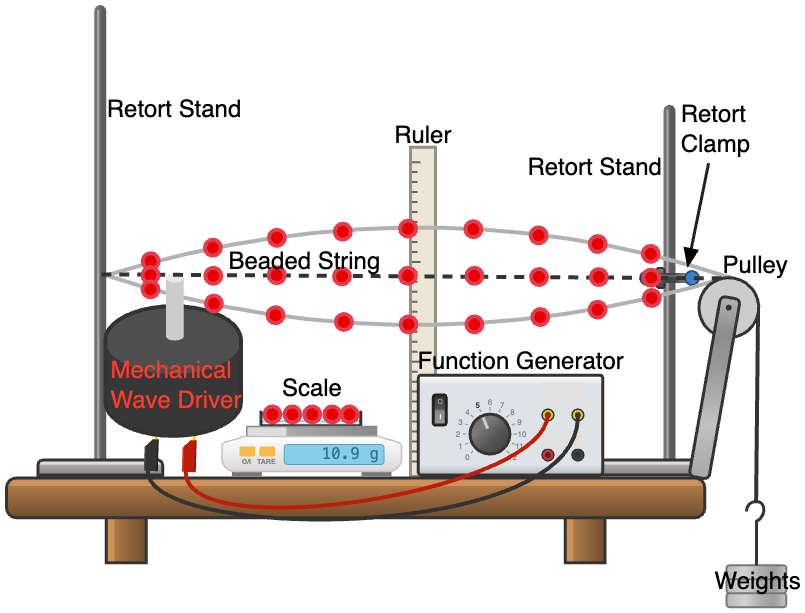
\includegraphics[width=4in]{images/setup.png}
    \caption{A diagram of our experimental setup}
    \label{fig:setup}
\end{figure}

% \pagebreak
\section{Procedure}

After this calibration, we tied one end of our string to the retort stand, and attempting to keep it level, we looped the other end over the pulley and tied on the weight hanger with 605 grams of weight (5.935 N of tension). We then placed the mechanical wave driver under the string so that the string rested in a notch in the driver's pronged extension. We then turned the function generator to 6 V and on the sine setting incremented by individual Hertz until the waves on the string appeared relatively stationary. We then incremented by tenths of a Hertz until the amplitude of the wave seemed largest, and recorded the frequency. However, it was tricky to get this calculation correct, as the modes seemed to be unstable equilibria, as the amplitude would increase until we incremented by just 0.1 Hz, and the whole thing collapsed. To keep this accurate we tried to find this point multiple times for each mode, and recorded the frequency before the standing wave collapsed. We did this for standing waves $n=1$ through $n=9$, the highest mode the string supports (similar to the Nyquist frequency, anything above this is impossible to measure).

Finally, we measured 9 beads to get an average mass we could use in our theoretical calculations.

\section{Results}

Unfortunately we were unable to measure each mode's wavelength via ruler, but we do know that our entire string was 100 cm long, so we can compute the wavelength from that measurement by $\frac{2\times100}{n}$, where $n$ is the mode. (This multiplication by 2 is due to the fact that we can only see half of the wave, not the entire thing.) To compute the velocity of each of the waves, we multiply the wavelength and the frequency ($\lambda \times f$), and propagate our errors using the equation (after we convert wavelength of $\frac{\text{m}}{\text{s}}$)

\begin{equation}
    \delta f^2=\sum_i \left(\frac{\delta f}{\delta a_i}\right)^2\delta a_i^2
\end{equation}

\begin{equation*}
    \delta v = \sqrt{\left(\frac{\delta v}{\delta f}\right)^2 \times 0.001 \text{ m}^2 + \left(\frac{\delta v}{\delta \lambda}\right)^2 \times 0.01 \text{ m}^2}=\sqrt{\left(\lambda\right)^2 \times 0.001 \text{ m}^2 + \left(f\right)^2 \times 0.01 \text{ m}^2}
\end{equation*}

We followed the same process to compute $k$, the angular wave number. $k=\frac{2\pi}{\lambda}$. We can also compute the angular frequency $\omega$ of the wave by $\omega=2\pi f$. All of that computed data, included propagated error, is present in Table \ref{tab:data}.

\begin{table}[]
\centering
\begin{tabular}{|l|l|l|l|l|l|}
\hline
      & Frequency     & Wavelength & Velocity & Wave Number& Angular Frequency \\ \hline
$n=1$ & 12.4 ± 0.1 Hz & 200 ± 1 cm & 24.80 ± 0.24 m/s & 3.14 ± 0.02 m$^{-1}$ & 77.91 ± 0.84 rad/s \\ \hline
$n=2$ & 24.6 ± 0.1 Hz & 100 ± 1 cm & 24.60 ± 0.27 m/s & 6.28 ± 0.06 m$^{-1}$ & 154.57 ± 2.27 rad/s \\ \hline
$n=3$ & 35.6 ± 0.1 Hz & 66 ± 1 cm & 23.50 ± 0.36 m/s & 9.52 ± 0.14 m$^{-1}$ & 223.68 ± 4.83 rad/s \\ \hline
$n=4$ & 44.2 ± 0.1 Hz & 50 ± 1 cm & 22.10 ± 0.44 m/s & 12.57 ± 0.25 m$^{-1}$ & 277.72 ± 7.88 rad/s \\ \hline
$n=5$ & 57.9 ± 0.1 Hz & 40 ± 1 cm & 23.16 ± 0.58 m/s & 15.71 ± 0.39 m$^{-1}$ & 363.80 ± 12.88 rad/s \\ \hline
$n=6$ & 64.7 ± 0.1 Hz & 34 ± 1 cm & 22.00 ± 0.65 m/s & 18.48 ± 0.54 m$^{-1}$ & 406.52 ± 16.92 rad/s \\ \hline
$n=7$ & 73.4 ± 0.1 Hz & 28 ± 1 cm & 20.55 ± 0.73 m/s & 22.44 ± 0.80 m$^{-1}$ & 461.19 ± 23.30 rad/s \\ \hline
$n=8$ & 75.5 ± 0.1 Hz & 26 ± 1 cm & 19.63 ± 0.76 m/s & 24.17 ± 0.93 m$^{-1}$ & 474.38 ± 25.81 rad/s \\ \hline
$n=9$ & 79.8 ± 0.1 Hz & 22 ± 1 cm & 17.56 ± 0.80 m/s & 28.56 ± 1.30 m$^{-1}$ & 501.40 ± 32.24 rad/s \\ \hline
\end{tabular}
\label{tab:data}
\caption{Data from $n=\{1\dots9\}$}
\end{table}

To see whether this data matched our theory, we plotted $\omega$ against $k$. We need to find a theoretical dispersion relation, which is helpfully derived in the supplemental resource (Berkeley Physics Course Vol. 3). See Equations \ref{eqn:dispersiontheo}-5 for this derivation. 

\begin{align}
\label{eqn:dispersiontheo}
    2 \cos (ka) &= 2- \frac{Ma}{T_0}\omega^2 \\
    \omega^2 &= \frac{2T_0}{Ma}\left[1-\left(\cos^2 \left(\frac{ka}{2}\right)-\sin^2 \left(\frac{ka}{2}\right)\right)\right] \\
    \omega^2 &= \frac{4T_0}{Ma} \sin^2 \left(\frac{ka}{2}\right) \\
    \omega(k) &= 2\sqrt{\frac{T_0}{Ma}}\sin\left(\frac{ka}{2}\right)
\end{align}


Using the final expression $\omega(k) = 2\sqrt{\frac{T_0}{Ma}}\sin\left(\frac{ka}{2}\right)$, we plot this with our actual data, plugging in our experimental values $T_0 = 5.935$ N, $a = 9$, and $m = 1$ g (which we computed from the mass of 9 beads, which was 10.38 g. Significant digits brings this to a nice 1 g). This gives us the final equation

\begin{equation}
\label{eqn:dispersion}
    \omega(k) = 2\sqrt{\frac{5.935 \text{ N}}{1 \text { g}\times 9 \text{ beads}}}\sin\left(\frac{k\times 9 \text{ beads}}{2}\right)
\end{equation}

Which we graphed from 0 to $\frac{\pi}{a}$, and overlaid on our $\omega$ vs $k$ plot, seen in Figure \ref{fig:frequency}. It looks good, with an $R^2$ of only 0.9891!

\begin{figure}[ht]
    \centering
    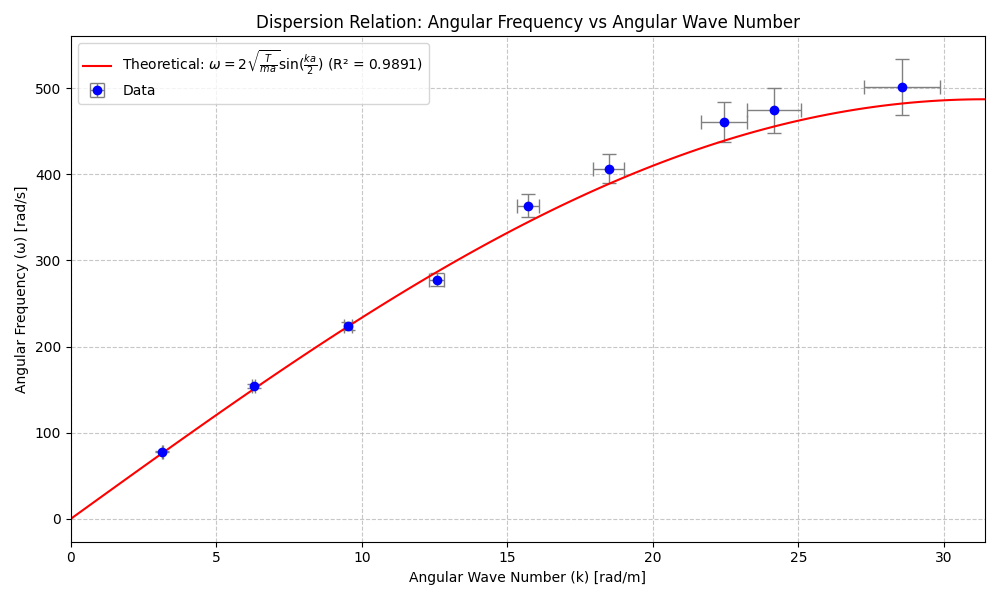
\includegraphics[width=7in]{images/dispersion_relation_filtered_with_errors.png}
    \caption{The wave number plotted against frequency with the theoretical fit}
    \label{fig:frequency}
\end{figure}

\section{Conclusions}

We were asked whether the dispersion relation between $\omega$ and $k$ was constant. From the data and theoretical fit, it seems conclusively not constant. If it weren't for the $\sin$ term, it would be a linear fit with no curve, but the beadedness of the string damps the modes frequency, and also makes for a non-constant velocity, as $v=\frac{\omega}{k}$, which are not changing linearly with each other.

\begin{figure}
    \centering
    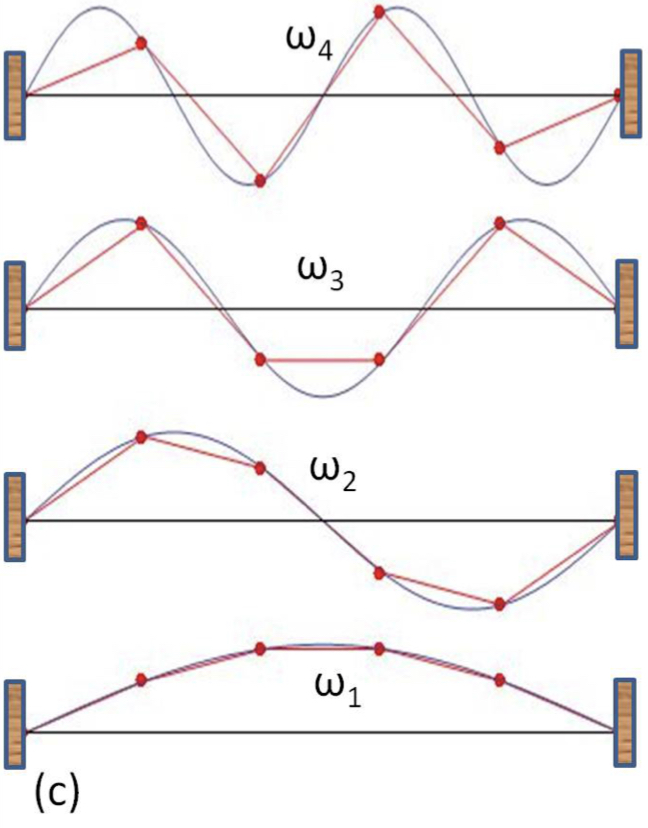
\includegraphics[width=3in]{images/beaded.jpg}
    \caption{Drawings of theoretical beaded string modes}
    \label{fig:beaded}
\end{figure}

% \bibliographystyle{unsrtnat}
% \bibliography{references}

\end{document}
